\section*{Aufgabe 3}

\subsection*{a)}
Gegeben $G=(N,\Sigma , P,S)$ mit $N=\{A,M,S,V,Z\}$ und $\Sigma = \{+,(,),0,1,2,x,y\}$ und $P=\{\\
S\rightarrow A+A|A ; A\rightarrow MV|Z|(S) ;\\
Z \rightarrow 0|1|2 ;\\ V \rightarrow x|y; \\
M \Rightarrow \varepsilon | Z\}$

Schritt 1:

Entfernen Von Epsilon Transitionen und Anwenden der Kettenregel:

$P'= \{\\S \rightarrow A+A| ZV|(S)|0|1|2|x|y;\\ A \rightarrow ZV|(S)|0|1|2|x|y;\\Z \rightarrow 0|1|2;\\ V \rightarrow x|y\}$

Schritt 2:

Einfügen neuer Nichtterminalsymbole:

$N'=\{A,S,S',V,Z,A_+,A_(,A_)\}$ und $P'= \{\\S \rightarrow AA_+A| ZV|A_(S'A_)|0|1|2|x|y;\\ A \rightarrow ZV|A_(S'A_)|0|1|2|x|y;\\Z \rightarrow 0|1|2;\\ V \rightarrow x|y;\\ A_+\rightarrow +;\\ A_( \rightarrow (;\\ A_) \rightarrow );\\ S' \rightarrow AA_+A| ZV|A_(S'A_)|0|1|2|x|y\}$

Schritt 3:

Verkürzen der Regeln:

$N'=\{A,S, S',V,Z,A_+,A_(,A_), B_1, B_2\}$ und $P'= \{\\S \rightarrow AB_1| ZV|A_(B_2|0|1|2|x|y;\\ A \rightarrow ZV|A_(B_2|0|1|2|x|y;\\Z \rightarrow 0|1|2; \\V \rightarrow x|y;\\ A_+\rightarrow +;\\ A_( \rightarrow (;\\ A_) \rightarrow );\\ S' \rightarrow AB_1| ZV|A_(B_2|0|1|2|x|y;\\ B_1 \rightarrow A_+A;\\ B_2 \rightarrow S'A_)\}$

Damit ist $G_c=(N',\Sigma, P',S)$ in Chomsky-Normalform und $L(G)=L(G_c)$

\subsection*{b)}
\begin{tabular}{c c c c c}
x & + & y & + & 1 \\
$SAVS'$ & $A_+$ & $SAVS'$ & $A_+$ & $SAZS'$ \\
$\emptyset$ & $B_1$ & $\emptyset$ & $ B_1$ &  \\
$SS'$ & $\emptyset$ & $SS'$ & &\\
$\emptyset$ & $\emptyset$ & & &\\
$\emptyset$ & & & &\\
\end{tabular}\\
S nicht in $V_{0,4}$ daher $x+y+1 \not\in L(G_c)$.\\



\begin{tabular}{c c}
2 & x \\
SAZS' & SAVS' \\
SAS' \\
\end{tabular}\\
S in $V_{0,1}$ daher $2x \in L(G_c)$

\subsection*{c)}
Sei N geordnet mit $N=\{S,S',B_1,A,B_2,V,Z,A_+,A_(,A_)\}$ \\
Erste Iteration:

Erste Anwendungen von (i):

$S \rightarrow AB_1| ZV|A_(B_2|0|1|2|x|y;\\
S' \rightarrow AB_1| ZV|A_(B_2|0|1|2|x|y;\\
B_1 \rightarrow A_+A;\\
A \rightarrow ZV|A_(B_2|0|1|2|x|y;\\
B_2 \rightarrow AB_1A_)| ZVA_)|A_(B_2A_)|0A_)|1A_)|2A_)|xA_)|yA_);\\
Z \rightarrow 0|1|2;\\
V \rightarrow x|y;\\ 
A_+\rightarrow +;
A_( \rightarrow (; 
A_) \rightarrow )$\\

Zweite Anwendung von (i):
$S \rightarrow AB_1| ZV|A_(B_2|0|1|2|x|y;\\
S' \rightarrow AB_1| ZV|A_(B_2|0|1|2|x|y;\\
B_1 \rightarrow A_+A;\\
A \rightarrow ZV|A_(B_2|0|1|2|x|y;\\
B_2 \rightarrow ZVB_1A_)|A_(B_2B_1A_)|0B_1A_)|1B_1A_)|2B_1A_)|xB_1A_)|yB_1A_)\\| ZVA_)|A_(B_2A_)|0A_)|1A_)|2A_)|xA_)|yA_);\\
Z \rightarrow 0|1|2;\\
V \rightarrow x|y;\\ 
A_+\rightarrow +;
A_( \rightarrow (; 
A_) \rightarrow )$\\


Zweite Iteration:

Erste Anwendung:

$S \rightarrow ZVB_1|A_(B_2B_1|0B_1|1B_1|2B_1|xB_1|yB_1| ZV|[B_2|0|1|2|x|y;\\
S' \rightarrow ZVB_1|A_(B_2B_1|0B_1|1B_1|2B_1|xB_1|yB_1| ZV|[B_2|0|1|2|x|y;\\
B_1 \rightarrow  +A;\\
A \rightarrow 0V|1V|2V|(B_2|0|1|2|x|y;\\
B_2 \rightarrow 0VB_1A_)|1VB_1A_)|2VB_1A_)|(B_2B_1A_)|0B_1A_)|1B_1A_)|2B_1A_)|xB_1A_)|yB_1A_)\\| 0VA_)|1VA_)|2VA_)|(B_2A_)|0A_)|1A_)|2A_)|xA_)|yA_);\\
Z \rightarrow 0|1|2;\\
V \rightarrow x|y;\\ 
A_( \rightarrow (; 
A_) \rightarrow )$\\

Zweite Anwendung:

$S \rightarrow 0VB_1|1VB_1|2VB_1|(B_2B_1|0B_1|1B_1|2B_1|xB_1|yB_1| 0V|1V|2V|(B_2|0|1|2|x|y;\\
S' \rightarrow 0VB_1|1VB_1|2VB_1|(B_2B_1|0B_1|1B_1|2B_1|xB_1|yB_1| 0V|1V|2V|(B_2|0|1|2|x|y;\\
B_1 \rightarrow  +A;\\
A \rightarrow 0V|1V|2V|(B_2|0|1|2|x|y;\\
B_2 \rightarrow 0VB_1A_)|1VB_1A_)|2VB_1A_)|(B_2B_1A_)|0B_1A_)|1B_1A_)|2B_1A_)|xB_1A_)|yB_1A_)\\| 0VA_)|1VA_)|2VA_)|(B_2A_)|0A_)|1A_)|2A_)|xA_)|yA_);\\
Z \rightarrow 0|1|2;\\
V \rightarrow x|y;\\ 
A_( \rightarrow (; 
A_) \rightarrow )$\\

Mit $P_G= \{S \rightarrow 0VB_1|1VB_1|2VB_1|(B_2B_1|0B_1|1B_1|2B_1|xB_1|yB_1| 0V|1V|2V|(B_2|0|1|2|x|y;\\
S' \rightarrow 0VB_1|1VB_1|2VB_1|(B_2B_1|0B_1|1B_1|2B_1|xB_1|yB_1| 0V|1V|2V|(B_2|0|1|2|x|y;\\
B_1 \rightarrow  +A;\\
A \rightarrow 0V|1V|2V|(B_2|0|1|2|x|y;\\
B_2 \rightarrow 0VB_1A_)|1VB_1A_)|2VB_1A_)|(B_2B_1A_)|0B_1A_)|1B_1A_)|2B_1A_)|xB_1A_)|yB_1A_)\\| 0VA_)|1VA_)|2VA_)|(B_2A_)|0A_)|1A_)|2A_)|xA_)|yA_);\\
Z \rightarrow 0|1|2;\\
V \rightarrow x|y;\\ 
A_( \rightarrow (; 
A_) \rightarrow ))\}$ 

Ist $G_g=\{N,\Sigma,P_G,S\}$ in Greibach-Normalform.
\subsection*{d)}

Sei K Kellerautomat wie folgt:\\
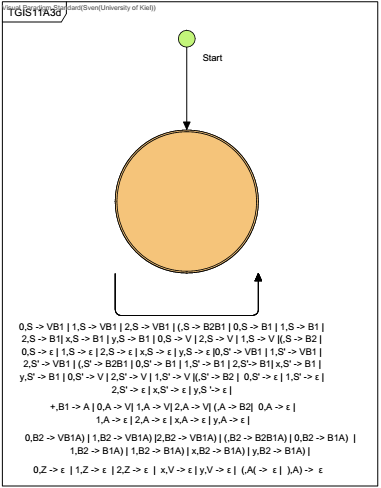
\includegraphics[width=\textwidth]{part/TGIS11A03d}\\
Mit K akzeptierend wenn des Speicher leer ist.
